% ============================================================
% 分片：s02f  对应原文 PDF 第 22--26 页
% 负责章节：§2 Twisting & mirror symmetry；2.3.4 Deformations；2.4 A brief introduction to homological mirror symmetry；2.4.1 Branes and categories in 2d TQFT
% 译者：translator-04   审校状态：初稿
% ============================================================
% [跨页接续: 原文第21页/22页。本分片自第22页第二段起；第22页首句
%  "where $\partial_\Sigma,\bar\partial_\Sigma$ are the worldsheet Dolbeault operators."
%  是对第21页式 (2.34) 的说明，按 SPEC §3 归 s02e。]
% [跨页接续: 末尾"见例如 [10, 第 2.5.3 节]；Kontsevich 还猜想……另见 [42, 43]。"一句
%  起于原文第26页末、止于第27页；本句按语义完整取于本分片，其后的
%  "We describe the construction ... in Section 3.2.3." 归 s02g。]

% ==== 原文 PDF 第 22 页 ====

与 $B$ 型扭变中的做法相同，可以得到局域算子的矢量空间。唯一 Lorentz 不变的选项必须由扭变后的世界面标量 $\phi,\bar\phi,\chi,\bar\chi$ 构造。其他任何可能通过用世界面度规缩并指标而构造出的假想标量，都会由于世界面度规的 $Q$-恰当性而成为 $Q$-恰当的。由于费米子场 $\chi,\bar\chi$ 取值于 $\mathcal{X}$ 的全纯与反全纯切丛，可以把它们等同于微分形式：

\begin{equation}
\chi^{n}\leftrightarrow \dd\phi^{n}\qquad \bar\chi^{\bar n}\leftrightarrow \dd\bar\phi^{\bar n}
\tag{2.35}
\end{equation}

于是 $Q_A$ 可自然地等同于作用于 $\mathcal{X}$ 上一般微分形式的 de Rham 微分
$d_{\mathcal{X}} = \dd\phi^{n}\,\partial_{\phi^{n}} + \dd\bar\phi^{\bar n}\,\partial_{\bar\phi^{\bar n}}$！
因此，$A$ 模型的局域算子可等同于靶流形的 de Rham 上同调：

% [Tutor Note: 这一步等同是 $A$ 型扭变的定义性要点：在算子--形式字典下扭变后的 $Q_A$ 与靶流形的 de Rham 微分 $d_{\mathcal{X}}$ 逐项对应，而世界面度规的 $Q$-恰当性保证一切含度规缩并的候选标量都不进入 $Q_A$ 上同调，故局域算子只依赖于靶流形的 de Rham 上同调类。B 模型取的是 Dolbeault 上同调，两者正是镜像对应的一侧。]
\begin{equation}
\text{局部算子的矢量空间：}\quad H^{\bullet}(\mathcal{X}) := H\bigl(\Omega^{(\bullet,\bullet)}(\mathcal{X}),\, d_{\mathcal{X}}\bigr).
\tag{2.36}
\end{equation}

与 $B$ 型扭变中一样，$A$ 型扭变具有 $\mathbb{Z}^2$-分次：$(p,q)$-形式的上同调次数 $C_A$（轴 $R$ 荷的负值）为 $p+q$，内部次数（矢量 $R$ 荷的负值）为 $p-q$。

% [Tutor Note: 易错预警：$C_A$ 定义为轴 $R$ 荷的负值，故 $(p,q)$-形式给出 $C_A=p+q$，而内部次数取矢量 $R$ 荷的负值、给出 $p-q$；两处负号来自扭变时 $U(1)_A$ 与 $U(1)_V$ 的混合。核对时应以式 (2.36) 中 $d_{\mathcal{X}}$ 使次数增加 $1$ 为基准，勿与后续章节的鬼数约定混淆。]

位于 $Q_A$ 局域化轨迹（localization locus，参见附录 A）中的映射 $\phi\colon\Sigma\to\mathcal{X}$ 满足 $\bar\partial_{\bar z}\phi=0$，因此拓扑 $A$ 模型局域化到靶空间的全纯映射。更具体地说，可以把扭变 $\sigma$ 模型的 Lagrange 量写成一个 $Q_A$-恰当项，再加上形如 $\int_{\phi(\Sigma)}\omega$ 的项——即靶空间（复化）凯勒类在世界面像上的积分，它只依赖于映射的同调类。该项只依赖于靶流形的凯勒类，而不依赖于其复结构，并且只依赖于世界面的同调类 $\beta=[\phi(\Sigma)]$。因此，$A$ 模型不仅在世界面上是拓扑的，而且在靶空间中是「半拓扑的」（half-topological）。所有对复结构的依赖都是 $Q_A$-恰当的。

% [Tutor Note: 推导补足：$A$ 模型的局域化来自 $Q_A$-恰当项 $\{Q_A,\cdot\}$；其玻色部分正比于 $\int_{\Sigma}|\bar\partial_{\bar z}\phi|^{2}$，故鞍点条件正是 $\bar\partial_{\bar z}\phi=0$，即全纯映射。另一方面 $\int_{\phi(\Sigma)}\omega$ 只看到同调类 $\beta=[\phi(\Sigma)]$，因此 $A$ 模型的关联函数只依赖于复化凯勒类的同调类代表，而不依赖于复结构。]

当 $\Sigma=S^{2}$ 时，这些映射通过手征环元素之间的关联函数，计算靶流形 $\mathcal{X}$ 中闭链的相交数。然而，非平凡的世界面瞬子（worldsheet instanton）可以对这些可观测量有贡献。它们是世界面 $\sigma$ 模型中的非微扰效应，因此 $A$ 模型是镜像对称对偶中「困难」的一侧。由 $A$ 模型中的关联函数，这些经量子修正的相交数与称为 Gromov--Witten 不变量（Gromov--Witten invariants）的计数不变量（enumerative invariants，粗略地说就是靶流形中全纯曲线的计数）相联系；后者本身已是代数几何中一个繁荣的研究领域。这些量子修正还形变微分形式的经典楔积：扭变手征环被等同于 $\mathcal{X}$ 的量子上同调（quantum cohomology）。关于这一主题的全面介绍，见例如 [9, 第 21--30 章]。镜像对称之所以有用，部分原因在于：在较简单的 $B$ 模型一侧作计算，可以用来提取 $A$ 一侧这些复杂的不变量。

% [Tutor Note: 物理图像：$A$ 模型只在世界面上是拓扑的，在靶空间中仍依赖全纯性，故称「半拓扑」；世界面瞬子（全纯曲线）给出非微扰修正，把经典楔积形变为量子上同调的乘积。镜像对称因此可以把 $A$ 一侧困难的 Gromov--Witten 计数转化为 $B$ 一侧的周期积分计算。]

\subsubsection{形变}

后文中我们将进一步讨论拓扑 $A$ 模型与 $B$ 模型中拓扑（即手征与扭手征）环所依赖的形变。正如所见，在 $A$ 模型情形，形变是靶空间凯勒模的函数；在 $B$ 模型情形则是复结构模的函数——对于在镜像对称下互换的量，这正是所预期的。两种情形下，形变都张成相应模空间的切丛；手征%
% ==== 原文 PDF 第 23 页 ====
环在几何模空间上给出有意思的丛，其中包含模空间的切丛作为子丛。

\subsection{同调镜像对称简介}

本节试图简要介绍同调镜像对称（homological mirror symmetry，HMS）的基本要素：上述扭变 Calabi--Yau $\sigma$ 模型中 $A$ 膜与 $B$ 膜的范畴。我们先回顾拓扑边界条件为何构成范畴，然后描述扭变 $\sigma$ 模型中膜的范畴。我们的目标是给出关于各种结构为何出现的直观理解，并非提供一部详尽的导引。更多细节，建议读者参阅综合性教科书 [9, 10] 及其中的文献。

\subsubsection{二维 TQFT 中的膜与范畴}

首先引入任何二维 TQFT 的核心对象：其边界条件的范畴。

范畴是许多数学分支的核心数学对象。简言之，范畴 $\mathcal{C}$ 是对象 $\operatorname{Obj}(\mathcal{C})$ 的集合，并对其每一对有序对象 $(B_1,B_2)\in\operatorname{Obj}(\mathcal{C})$ 给出态射 $\Hom_{\mathcal{C}}(B_1,B_2)$，连同复合态射的规则

% [Tutor Note: 式 (2.37) 把范畴的复合律画成一个映射：第一行是 Hom 空间之间的映射，第二行的 $\ni$、$\in$ 标出各集合的元素归属，第三行是元素层面的对应。注意复合写作 $O_{23}O_{12}$，即先作用 $O_{12}$ 再作用 $O_{23}$（从右向左），与算子乘积的书写次序一致。]
\begin{equation}
\begin{array}{c@{\quad}c@{\quad}c@{\quad}c@{\quad}c} \Hom_{\mathcal{C}}(B_1,B_2) & \times & \Hom_{\mathcal{C}}(B_2,B_3) & \longrightarrow & \Hom_{\mathcal{C}}(B_1,B_3)\\[2pt]
\ni & & \ni & & \in\\[2pt] O_{12} & & O_{23} & \mapsto & O_{23}O_{12}\end{array}\tag{2.37}
\end{equation}

此外，态射的复合要求满足结合性\footnote{如第 3.2 节所述，态射的结合性可以放宽为同伦意义下的结合性。本节中我们只关注严格结合的态射复合。}：若给定态射 $O_{ij}\in\Hom_{\mathcal{C}}(B_i,B_j)$，则 $O_{34}(O_{23}O_{12})=(O_{34}O_{23})O_{12}$。读者可能熟悉的一些范畴例子如下：

\begin{enumerate}
\item \textbf{Set}：集合的范畴；\textbf{Set} 的对象是集合，态射是函数。
\item \textbf{Top}：拓扑空间的范畴；\textbf{Top} 的对象是拓扑空间，态射是同胚。
% [原文疑误: 拓扑空间范畴 \textbf{Top} 的态射应为连续映射，而非同胚；同胚只是其中可逆的态射。建议改为「态射是连续映射」。]
\item \textbf{Grp}：群的范畴；\textbf{Grp} 的对象是群，态射是群同态。
\item $\mathrm{Rep}(G)$：群 $G$ 的表示范畴；对象是 $G$ 的表示，态射是缠绕算子（intertwining operator）。
\end{enumerate}

我们断言：二维 TQFT 中的边界条件具有范畴的结构。更一般地，在任意 $d$ 维 TQFT 中，支撑在时空的一维子流形上的延展算子——称为线算子（line operator）或线缺陷（line defect）——具有这样的结构。再更一般地，此类理论中支撑为 $k$ 维的算子具有 $k$-范畴的结构，这需要给出%
% ==== 原文 PDF 第 24 页 ====
同一对对象（0-态射）之间的任意一对态射（也称 1-态射）之间的 2-态射的数据，如此直至适当的 $(k-1)$-态射对之间的 $k$-态射。

二维 TQFT $\mathcal{T}$ 的边界条件范畴 $\mathbf{Bdy}$ 的构造如下：$\mathbf{Bdy}$ 中的对象是 $\mathcal{T}$ 所允许的边界条件 $B$。给定两个边界条件 $B_1,B_2$，态射 $O_{12}\in\Hom_{\mathbf{Bdy}}(B_1,B_2)$ 是边界上在 $B_1$ 与 $B_2$ 之间插值的局域算子。态射的复合由边界局域算子的碰撞（collision）诱导；见图 2。对于高维 TQFT 中线算子的范畴，也有类似的图景。高维缺陷的高阶范畴结构来自考虑不同维数的交汇处（junction）；例如，面算子（二维支撑）构成一个 2-范畴，其 1-态射是连接两个面算子的线算子，其 2-态射是连接此类线算子的局域算子。更详尽的介绍见例如 [39] 及其中的文献。

% [Tutor Note: 推导补足：边界局域算子的碰撞即 OPE 的极限，态射复合的结合性 $O_{34}(O_{23}O_{12})=(O_{34}O_{23})O_{12}$ 对应同一次三点碰撞的不同结合顺序；在严格结合的情形这是等号，而在 $A_\infty$ 或导出框架中只要求同伦结合（见第 3.2 节）。]
\begin{figure}[tbp]
  \centering
  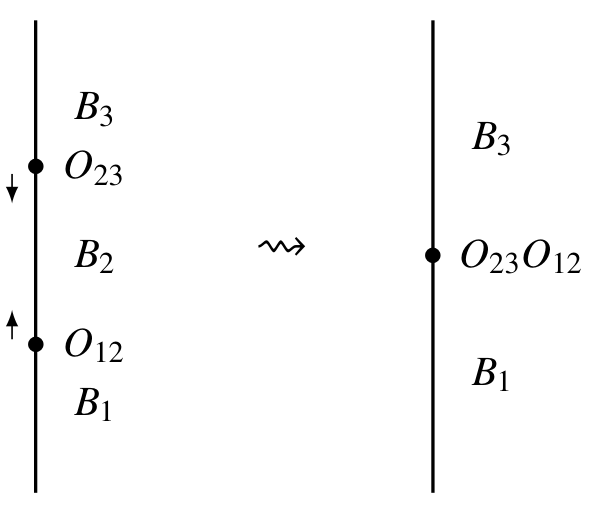
\includegraphics[width=0.92\linewidth]{figures/fig02.png}
  \caption{二维 TQFT 中边界条件范畴里态射的复合示意：它由边界局域算子的碰撞诱导。
  （原文第 24 页，Figure 2）}
\end{figure}

通过一些标准的 TQFT 操作，可以得到这一态射空间的另外两种诠释。第二种描述使用态--算子对应：边界局域算子 $O_{12}\in\Hom_{\mathbf{Bdy}}(B_1,B_2)$ 在围绕插入点的半圆弧（或任何其他同调的闭链）上产生一个态；反之，这样一个半圆上的态在弧长趋于无穷小的极限下产生一个局域算子；见图 3 中图。第三种描述利用理论的拓扑性质，通过复对数将该半空间形变为一条长条。在此映射下，半圆弧被映为长条中的一条水平线，从而把半圆上的态映为长条上的态；见图 3 右图。

\begin{figure}[tbp]
  \centering
  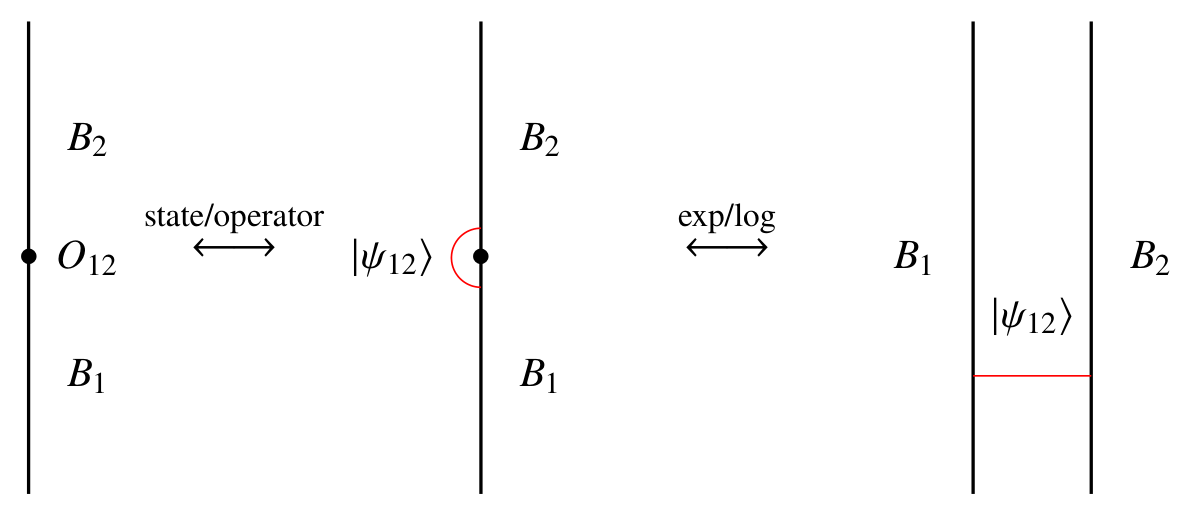
\includegraphics[width=0.92\linewidth]{figures/fig03.png}
  \caption{态射空间 $\Hom_{\mathbf{Bdy}}(B_1,B_2)$ 的三种诠释。左：在 $B_1$ 与 $B_2$ 之间插值的局域算子。中：锚定在两个边界条件 $B_1,B_2$ 上的半圆上的态。右：两端边界条件为 $B_1,B_2$ 的长条上的态。
  （原文第 25 页，Figure 3）}
\end{figure}

最后这种描述自然地给出弦论诠释：两个膜 $B_1,B_2$ 之间的态射空间被等同于开弦态的空间，开弦的两端满足相应的边界条件。在此诠释下，态射的复合来自开弦的拼接；见图 4。

\begin{figure}[tbp]
  \centering
  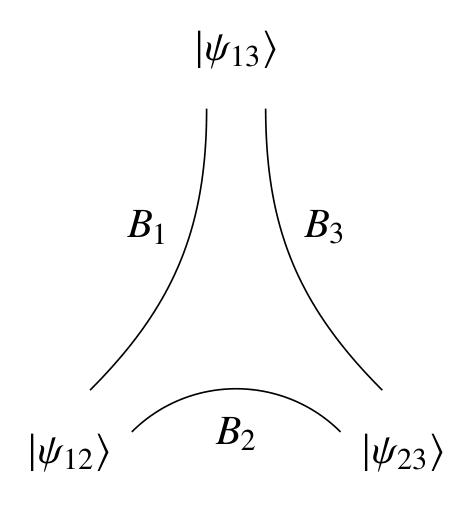
\includegraphics[width=0.92\linewidth]{figures/fig04.png}
  \caption{以开弦拼接的方式图示边界条件范畴中态射的复合。
  （原文第 25 页，Figure 4）}
\end{figure}

事实证明，边界条件的范畴足够丰富，可以通过其 Hochschild 上同调重构第 2.3 节所描述的闭弦部分，参见 [10, 第 2.2.3 节] 或 [40] 及其中的文献。\footnote{严格地说，与拓扑弦相关的是循环上同调（cyclic cohomology）。循环上同调对应于循环对称的 Hochschild 上链的上同调；这一循环对称性要求与如下事实相关：弦论将 TQFT 与拓扑引力耦合，因此必须对边界插入的模进行积分。在未与引力耦合的情形，相关的是完整的上同调。} 论证如下。\footnote{我们采取的视角与 [10, 第 2.2.3 节] 的精神一致。关于体局域算子与 Hochschild 上同调的等同，另一种有用的视角借助折叠技巧（folding trick），参见 [40]。这相当于把二维理论 $\mathcal{T}$ 中的体局域算子看成束缚在 $\mathcal{T}$ 与自身之间「平凡界面」上的局域算子；等价地，体局域算子可视为 $\mathcal{T}\times\mathcal{T}^{-}$ 中对角膜上的边界局域算子，其中 $\mathcal{T}^{-}$ 由 $\mathcal{T}$ 沿边界反射得到。} 若 $O$ 是体%
% ==== 原文 PDF 第 25 页 ====
局域算子，且 $B$ 是拓扑膜，则可将 $O$ 移到边界上，得到（可能为零的）边界局域算子 $O|_B$，即态射 $O|_B\in\Hom_{\mathbf{Bdy}}(B,B)$。此外，膜 $B_1$ 与 $B_2$ 之间的态射空间 $\Hom_{\mathbf{Bdy}}(B_1,B_2)$ 通过碰撞自然地成为体局域算子的模，即得到映射 $O\colon \Hom_{\mathbf{Bdy}}(B_1,B_2)\to\Hom_{\mathbf{Bdy}}(B_1,B_2)$，其中 $O_{12}\mapsto O\cdot O_{12}$。可以把边界局域算子 $O|_B$ 视为 $O\cdot \operatorname{id}_B$，其中 $\operatorname{id}_B$ 是 $B$ 上的恒等算子。由于体局域算子可以自由地碰撞在边界上的任何位置，由此可知这两种操作相互交织：

% [Tutor Note: 易错预警：式 (2.38) 表明体算子从边界两侧作用的结果一致，这正是 $O|_B$ 位于边界算子代数中心（即与 $A$ 中所有元素对易）的来源；注意左右两端的下标 $B_2$、$B_1$ 不可互换。]
\begin{equation}
O|_{B_2}O_{12} = (O\cdot O_{12}) = O_{12}O|_{B_1}.
\tag{2.38}
\end{equation}

见图 5。

\begin{figure}[tbp]
  \centering
  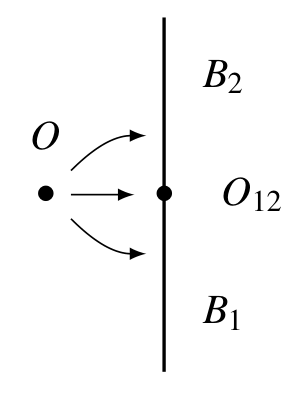
\includegraphics[width=0.92\linewidth]{figures/fig05.png}
  \caption{两个边界条件交汇处的局域算子必须与体局域算子的作用对易；而且它们本身构成体局域算子代数上的模结构。
  （原文第 26 页，Figure 5）}
\end{figure}

用范畴的语言说，满足这些关系的映射族 $\{O|_B\}$ 是恒等自函子 $\operatorname{id}_{\mathbf{Bdy}}\colon \mathbf{Bdy}\to\mathbf{Bdy}$ 的自然变换。下面解析这一陈述。首先，（协变）函子是范畴之间的一类映射 $\mathcal{F}\colon \mathcal{C}_1\to\mathcal{C}_2$（又称范畴的 2-范畴中的 1-态射）。$\mathcal{F}$ 的数据包括对象上的映射

\begin{equation}
B\in\operatorname{Obj}(\mathcal{C}_1)\mapsto \mathcal{F}(B)\in\operatorname{Obj}(\mathcal{C}_2)
\tag{2.39}
\end{equation}

% ==== 原文 PDF 第 26 页 ====
以及任意两个对象 $B_1,B_2$ 之间态射上的映射

\begin{equation}
O_{12}\in\Hom_{\mathcal{C}_1}(B_1,B_2)\mapsto \mathcal{F}(O_{12})\in\Hom_{\mathcal{C}_2}\bigl(\mathcal{F}(B_1),\mathcal{F}(B_2)\bigr).
\tag{2.40}
\end{equation}

此外，这些映射与态射的复合相容；给定 $O_{12}\in\Hom_{\mathcal{C}_1}(B_1,B_2)$ 与 $O_{23}\in\Hom_{\mathcal{C}_1}(B_2,B_3)$，在 $\Hom_{\mathcal{C}_2}(\mathcal{F}(B_1),\mathcal{F}(B_3))$ 中有如下等式：

\begin{equation}
\mathcal{F}(O_{23}O_{12}) = \mathcal{F}(O_{23})\mathcal{F}(O_{12}).
\tag{2.41}
\end{equation}

自函子就是从范畴到自身的函子；恒等自函子 $\operatorname{id}_{\mathbf{Bdy}}$ 是 $\mathbf{Bdy}$ 的「什么都不做」的自函子

\begin{equation}
\operatorname{id}_{\mathbf{Bdy}}(B) = B \qquad \operatorname{id}_{\mathbf{Bdy}}(O_{12}) = O_{12}.
\tag{2.42}
\end{equation}

最后，自然变换是函子之间的映射 $\eta\colon \mathcal{F}\to\mathcal{G}$（又称范畴的 2-范畴中的 2-态射）。它由对每个对象 $B\in\operatorname{Obj}(\mathcal{C}_1)$ 的映射 $\eta_B\colon \mathcal{F}(B)\to\mathcal{G}(B)$ 的数据给出，这些映射与态射的映射相互交织

\begin{equation}
\eta_{B_2}\mathcal{F}(O_{12}) = \mathcal{G}(O_{12})\eta_{B_1}\in\Hom_{\mathcal{C}_2}\bigl(\mathcal{F}(B_1),\mathcal{G}(B_2)\bigr).
\tag{2.43}
\end{equation}

取函子 $\mathcal{F}$ 与 $\mathcal{G}$ 为恒等自函子，即见式 (2.38) 恰好是如下陈述：体局域算子 $O$ 定义了从 $\operatorname{id}_{\mathbf{Bdy}}$ 到自身的自然变换。

考虑范畴具有（或更一般地，由之生成）单个边界条件 $B$ 的情形。于是只需考虑 $B$ 上局域算子的代数 $A$，即 $A=\Hom_{\mathbf{Bdy}}(B,B)$。那么，对每个体局域算子 $O$，都有元素 $O|_B\in A$；式 (2.38) 表明 $O|_B$ 与 $A$ 中其他每个元素对易，即 $O|_B$ 属于 $A$ 的中心，$O|_B\in Z(A)$。但这不可能就是全部，因为例如非平凡的体局域算子移到边界上可能为零。在完全导出的框架下，例如当所考虑的 TQFT 经由扭变得到、或采用 BV 形式时，$A$ 的中心只是 $A$ 的完整 Hochschild 上同调（系数在 $A$ 中）的第零上同调群，或简单说就是 $A$ 的导出中心：$Z(A)\cong \HH^{0}(A)\subset\HH^{\bullet}(A)$。对于具有更精细拓扑膜范畴的理论，存在自然的推广，即得到膜的范畴的 Hochschild 上同调 $\HH^{\bullet}(\mathbf{Bdy})$。体局域算子与拓扑膜范畴的 Hochschild 上同调之间的等同，被预期在相当一般的情形下成立。

% [Tutor Note: 推导补足：把体局域算子视为 Hochschild 上链，其插入点在边界上的循环次序给出上闭链（cocycle）条件；与拓扑引力耦合后需要对所有边界插入点的模作积分，故相关的是循环上同调（见脚注）。而导出中心 $Z(A)\cong \HH^{0}(A)$ 只是 $\HH^{\bullet}(A)$ 的最低阶部分。]
例如，已知它能从 $B$ 膜的范畴恢复第 2.3.2 节所描述的整个 $\sigma$ 模型手征环，见例如 [10, 第 2.5.3 节]；Kontsevich 还猜想，对于（困难得多的）$A$ 膜范畴，同样的事实应当成立 [41]，另见 [42, 43]。

% [Tutor Note: 物理图像：同调镜像对称（HMS）猜想把 $A$ 膜范畴（辛几何一侧的 Fukaya 范畴）与 $B$ 膜范畴（复几何一侧的凝聚层导出范畴）等同起来，于是镜像对称在范畴层面成为同调代数中的等价。这正是下一小节分别讨论两类膜的原因。]

% [本分片至此结束。下一句 "We describe the construction of Hochschild cohomology ...
%  in Section 3.2.3." 起于原文第27页，见 s02g 开头。]
